\subsubsection{Malha de corrente}

O estudo da malha de corrente para esta situação é o mesmo para o caso do controle em cascata esboçado na seção anterior.

\subsubsection{Malha de velocidade}

A malha de velocidade pode ser representada pelo diagrama da figura \ref{fig:D1_62}. Dado que $L_{a} = 0$ (pequenas perturbações).

\begin{figure}[ht!]
\center
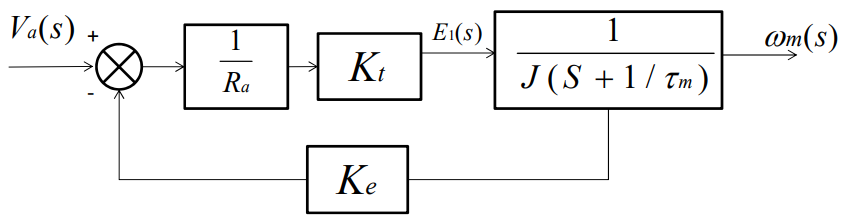
\includegraphics[scale= 0.55]{imagens/diagrama1_62.png}
\caption{\label{fig:D1_62} Diagrama de blocos do motor da malha de velocidade considerando $L_{a} = 0$.}
\caption*{Fonte: MARTINS, cap. 3, eslaide 14.}
\end{figure}

Assim:
\[\frac{\omega_{m}(s)}{V_{a}(s)} = \frac{K_{t}/R_{a}J}{\left(s + 1/\tau_{m2}\right)}\]
\[\tau_{m2} = \frac{\tau_{m1}\tau_{m}}{\tau_{m1} + \tau_{m}}\]
\[\tau_{m1} = \frac{R_{a}J}{K_{e}K_{t}}\]

Portanto, o diagrama de blocos pode ser representado como na figura \ref{fig:D2_62}.

\begin{figure}[ht!]
\center
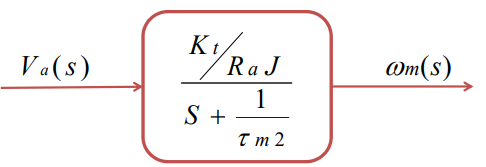
\includegraphics[scale= 0.55]{imagens/diagrama2_62.png}
\caption{\label{fig:D2_62} Diagrama de blocos do motor}
\caption*{Fonte: MARTINS, cap. 3, eslaide 15.}
\end{figure}

A figura \ref{fig:D3_62} representa o diagrama com o conversor e o regulador proporcional - integral inclusos.

\begin{figure}[ht!]
\center
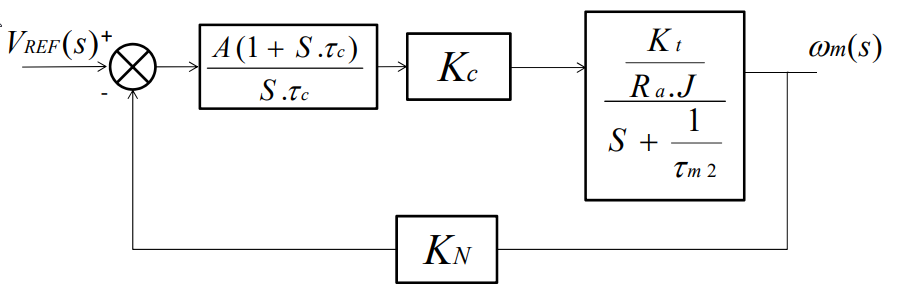
\includegraphics[scale= 0.55]{imagens/diagrama3_62.png}
\caption{\label{fig:D3_62} Diagrama de blocos do motor CC incluindo o conversor estático e o regulador.}
\caption*{Fonte: MARTINS, cap. 3, eslaide 16.}
\end{figure}

A função de transferência é representada pela seguinte expressão:

\[\frac{\omega_{m}(s)}{V_{REF}(s)} = \frac{1 + s\tau_{C}/K_{N}}{1 + s\tau_{C}\left(1 + \frac{R_{a}J}{A.K_{C}.K_{I}.K_{N}\tau_{m2}}\right) +\frac{R_{a}J\tau{C}s^{2}}{AK_{C}K_{t}K_{N}}}\]

Seja,
\[\frac{R_{a}J}{AK_{C}K_{t}K_{N}\tau_{m2}} << 1\]
\[\tau_{3} = \frac{R_{a}J}{AK_{C}K_{t}K_{N}} \]

Assim:

\[\frac{W_{m}(s)}{V_{REF}(s)} = \frac{\left(1 + s\tau_{C}/K_{N}\right)}{\tau_{C}\tau_{3}s^{2} + \tau_{C}s + 1}\]

A equação característica é:
\[s^{2} + \frac{s}{\tau_{3}} + \frac{1}{\tau_{3}\tau_{C}} = 0\]
\[2\alpha = \frac{1}{\tau_{3}}\]
\[\omega_{n}^{2} = \frac{1}{\tau_{3}\tau_{C}}\]
\[\epsilon = \frac{\alpha}{\omega_{n}} = \frac{1}{2\tau_{3}}\sqrt{\tau_{3}\tau_{C}} = \frac{1}{2}\sqrt{\frac{\tau_{C}}{\tau_{3}}}\]
\[\epsilon = 0,707\]
\[\tau_{C} = 2\tau_{3}\]
\[\tau_{3} = \frac{1}{W_{m}\sqrt{2}}\]
\[A = \frac{R_{a}J}{K_{C}K_{t}K_{N}\tau_{3}}\]

Dessa forma pode-se calcular o regulador de velocidade.

